\documentclass[a4paper,12pt]{article}

\usepackage{fancyhdr}
\usepackage{lastpage}
\usepackage{amsmath}
\usepackage{tikz}
\usepackage{amsfonts}
\usepackage{csvsimple}
\usepackage{graphicx}


\newcommand{\V}[1]{\ensuremath{\vec{#1}}}
\newcommand{\F}[2]{\ensuremath{\frac{#1}{#2}}}
\newcommand{\Q}[1]{\newpage \section*{#1}}
\newcommand{\acc}[1]{\overset{..}{#1}}
\newcommand{\vel}[1]{\overset{.}{#1}}
\newcommand{\prt}[2]{\frac{\partial#1}{\partial#2}}
\newcommand{\LP}{\left(}
\newcommand{\RP}{\right)}

\pagestyle{fancy}
\lhead{Samuel Loomis}
\setlength{\headheight}{15pt}
\chead{Electromagnetism HW 2}
\rhead{\thepage\ of \pageref{LastPage}}
\lfoot{}
\cfoot{}
\rfoot{}

\begin{document}

\subsection*{Question 1}
What is the bound charge distribution of an infinately long uniformly polarized equilateral triangle whose polarization is $\V{P}$. What is the total bound charge? What is the far field electric field produced by the triangle?
\begin{figure}[h]
\centering
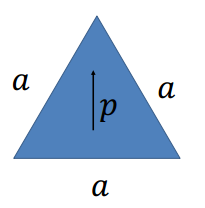
\includegraphics{Triangle-Dielectric.png}
\end{figure}\\
Intuitively, the positive charges will be accumulate at the top of the triangle and the negative charges will accumulate at the bottom. \\
\\
The mathematical representation for the surface bound charge density is:
\[\sigma_b=P\cdot\hat{n}\]
For this triangular solid there are three normal vectors to solve for.  Measuring from $\theta=0$ pointing in the $\hat{z}$, the three normal vectors are: $\hat{n}_1: \theta_1=\F{-\pi}{3}, \hat{n}_2:\theta_2=\F{\\pi}{3}, and \hat{n}_3:\theta_3=\pi$.\\
\\
Solving for the surface bound charge densities:
\begin{align*}
\sigma_{b1}=P\cdot\hat{n}_1=Pcos\LP\F{-\pi}{3}\RP=\F{P}{2}\\
\sigma_{b2}=P\cdot\hat{n}_2=Pcos\LP\F{\pi}{3}\RP=\F{P}{2}\\
\sigma_{b3}=P\cdot\hat{n}_3=Pcos(\pi)=-P
\end{align*}\\
The volume charge density is equal to the negative divergance of the polarization, and the divergance of a uniform polarization is 0, so $\rho_b$ for this material is 0.\\
\\
To find the far field electric field created by this arrangement...  the potential due to a surface charge density is:
\[V(r)=\F{1}{4\pi\epsilon_0}\int_S\F{\sigma_n}{r-r'}da'\]
$\sigma_1$:
\begin{align*}
r'_1(t)=\LP\F{a}{2}t-\F{a}{2}\RP\hat{x}+\F{\sqrt{3}}{2}at\hat{z}
\end{align*}
$\sigma_2$:
\[r'_2(t)=\F{a}{2}t\hat{x}+\LP-\F{\sqrt{3}}{2}at+\F{\sqrt{3}}{2}a\RP\hat{z}\]
$\sigma_3$:
\[r'_3(t)=\LP at-\F{a}{2}\RP\hat{x}\]

\Q{Question 2}
Read the example given in Griffiths (Example 4.7) for a dielectric material in uniform electric field.  And consider the following problem: a sphere of dielectric constant $\epsilon_r^1$ is placed inside dielectric material of $\epsilon_r^2$.  Now a uniform electric field is applied externally.  Solve for the electric field inside and outside of the sphere.  What is the charge density at the interface?  Prove that the $\V{E_\theta}$ is continuous cross the interface.  What is the difference between $\V{D_\theta}$ inside and outside the sphere?

\end{document}


